

\tikzset{every picture/.style={line width=0.75pt}} %set default line width to 0.75pt        

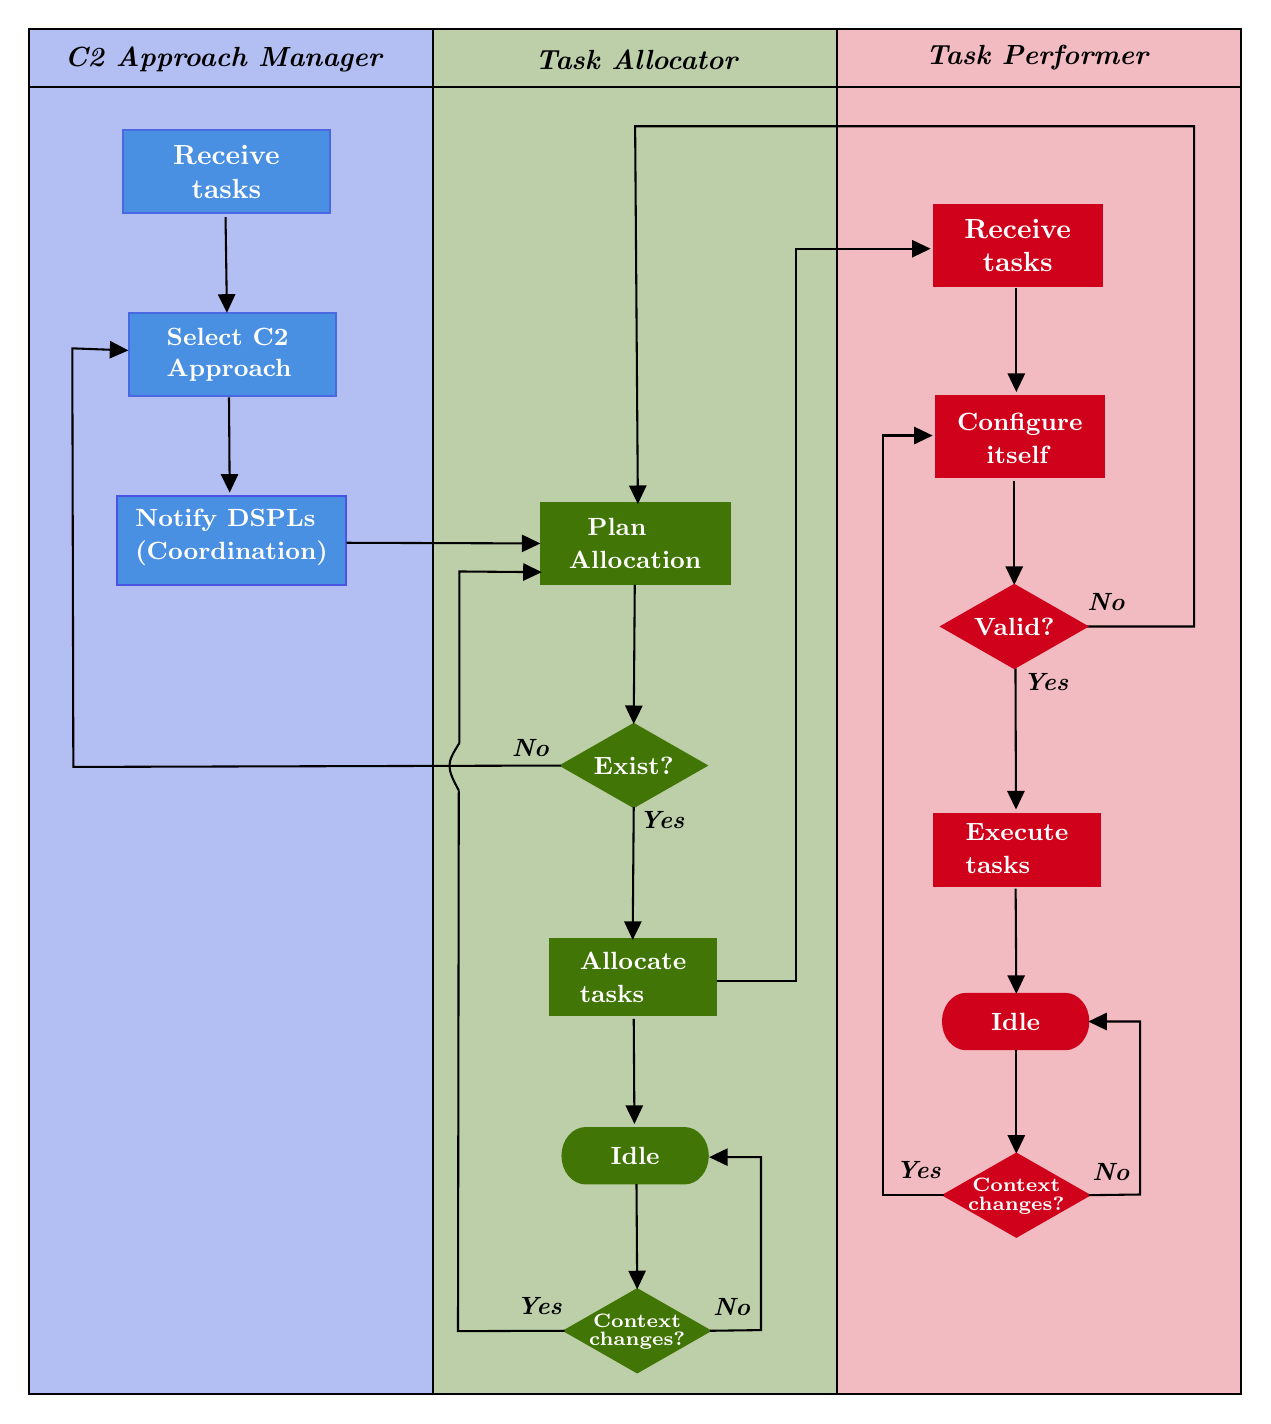
\begin{tikzpicture}[x=0.75pt,y=0.75pt,yscale=-1,xscale=1]
%uncomment if require: \path (0,673); %set diagram left start at 0, and has height of 673

%Shape: Rectangle [id:dp8854253159391561] 
\draw  [fill={rgb, 255:red, 74; green, 102; blue, 226 }  ,fill opacity=0.42 ] (2.5,3) -- (197.5,3) -- (197.5,661) -- (2.5,661) -- cycle ;
%Shape: Rectangle [id:dp3469463448197052] 
\draw  [fill={rgb, 255:red, 65; green, 117; blue, 5 }  ,fill opacity=0.35 ] (197.5,3) -- (392,3) -- (392,661) -- (197.5,661) -- cycle ;
%Shape: Rectangle [id:dp018917795120609204] 
\draw  [fill={rgb, 255:red, 208; green, 2; blue, 27 }  ,fill opacity=0.27 ] (392,3) -- (586.67,3) -- (586.67,661) -- (392,661) -- cycle ;
%Straight Lines [id:da8146359528310543] 
\draw    (2.5,31) -- (587,31) ;
%Flowchart: Process [id:dp15412574148578628] 
\draw  [color={rgb, 255:red, 74; green, 104; blue, 226 }  ,draw opacity=1 ][fill={rgb, 255:red, 74; green, 144; blue, 226 }  ,fill opacity=1 ] (51,140) -- (150.5,140) -- (150.5,180) -- (51,180) -- cycle ;
%Flowchart: Process [id:dp48065105856176205] 
\draw  [color={rgb, 255:red, 74; green, 83; blue, 226 }  ,draw opacity=1 ][fill={rgb, 255:red, 74; green, 144; blue, 226 }  ,fill opacity=1 ] (45,228.17) -- (155.5,228.17) -- (155.5,270.83) -- (45,270.83) -- cycle ;
%Flowchart: Process [id:dp6629894570275567] 
\draw  [color={rgb, 255:red, 65; green, 117; blue, 5 }  ,draw opacity=1 ][fill={rgb, 255:red, 65; green, 117; blue, 5 }  ,fill opacity=1 ] (249.17,231.33) -- (340.17,231.33) -- (340.17,270.33) -- (249.17,270.33) -- cycle ;
%Flowchart: Decision [id:dp5160918625824323] 
\draw  [color={rgb, 255:red, 65; green, 117; blue, 5 }  ,draw opacity=1 ][fill={rgb, 255:red, 65; green, 117; blue, 5 }  ,fill opacity=1 ] (294,338) -- (329,358) -- (294,378) -- (259,358) -- cycle ;
%Flowchart: Process [id:dp8044553855974566] 
\draw  [color={rgb, 255:red, 65; green, 117; blue, 5 }  ,draw opacity=1 ][fill={rgb, 255:red, 65; green, 117; blue, 5 }  ,fill opacity=1 ] (253.67,441.67) -- (333.67,441.67) -- (333.67,478.33) -- (253.67,478.33) -- cycle ;
%Straight Lines [id:da6701074801455137] 
\draw    (259,358) -- (24,358.67) -- (23.5,157) -- (47.5,157.89) ;
\draw [shift={(50.5,158)}, rotate = 182.12] [fill={rgb, 255:red, 0; green, 0; blue, 0 }  ][line width=0.08]  [draw opacity=0] (8.93,-4.29) -- (0,0) -- (8.93,4.29) -- cycle    ;
%Straight Lines [id:da6383024146874764] 
\draw    (294,378) -- (293.52,439) ;
\draw [shift={(293.5,442)}, rotate = 270.45] [fill={rgb, 255:red, 0; green, 0; blue, 0 }  ][line width=0.08]  [draw opacity=0] (8.93,-4.29) -- (0,0) -- (8.93,4.29) -- cycle    ;
%Straight Lines [id:da7026427833669057] 
\draw    (294.5,271) -- (294.02,335) ;
\draw [shift={(294,338)}, rotate = 270.43] [fill={rgb, 255:red, 0; green, 0; blue, 0 }  ][line width=0.08]  [draw opacity=0] (8.93,-4.29) -- (0,0) -- (8.93,4.29) -- cycle    ;
%Straight Lines [id:da7965236156041576] 
\draw    (155.67,250.67) -- (246,250.99) ;
\draw [shift={(249,251)}, rotate = 180.2] [fill={rgb, 255:red, 0; green, 0; blue, 0 }  ][line width=0.08]  [draw opacity=0] (8.93,-4.29) -- (0,0) -- (8.93,4.29) -- cycle    ;
%Straight Lines [id:da4788721755855869] 
\draw    (97.33,93.83) -- (97.96,136.83) ;
\draw [shift={(98,139.83)}, rotate = 269.17] [fill={rgb, 255:red, 0; green, 0; blue, 0 }  ][line width=0.08]  [draw opacity=0] (8.93,-4.29) -- (0,0) -- (8.93,4.29) -- cycle    ;
%Straight Lines [id:da7999024493741219] 
\draw    (99,180.67) -- (99.31,223.5) ;
\draw [shift={(99.33,226.5)}, rotate = 269.58] [fill={rgb, 255:red, 0; green, 0; blue, 0 }  ][line width=0.08]  [draw opacity=0] (8.93,-4.29) -- (0,0) -- (8.93,4.29) -- cycle    ;
%Shape: Rectangle [id:dp4479174596462915] 
\draw  [color={rgb, 255:red, 208; green, 2; blue, 27 }  ,draw opacity=1 ][fill={rgb, 255:red, 208; green, 2; blue, 27 }  ,fill opacity=1 ] (439.5,180) -- (520.5,180) -- (520.5,219) -- (439.5,219) -- cycle ;
%Flowchart: Process [id:dp18610523674883006] 
\draw  [color={rgb, 255:red, 208; green, 2; blue, 27 }  ,draw opacity=1 ][fill={rgb, 255:red, 208; green, 2; blue, 27 }  ,fill opacity=1 ] (438.67,381.33) -- (518.67,381.33) -- (518.67,416) -- (438.67,416) -- cycle ;
%Flowchart: Terminator [id:dp6793353293966301] 
\draw  [color={rgb, 255:red, 208; green, 2; blue, 27 }  ,draw opacity=1 ][fill={rgb, 255:red, 208; green, 2; blue, 27 }  ,fill opacity=1 ] (454.2,468) -- (501.8,468) .. controls (507.99,468) and (513,473.97) .. (513,481.33) .. controls (513,488.7) and (507.99,494.67) .. (501.8,494.67) -- (454.2,494.67) .. controls (448.01,494.67) and (443,488.7) .. (443,481.33) .. controls (443,473.97) and (448.01,468) .. (454.2,468) -- cycle ;
%Straight Lines [id:da16428269292090503] 
\draw    (512.33,291) -- (564,291) -- (564,50) -- (294.67,50) -- (295.98,229) ;
\draw [shift={(296,232)}, rotate = 269.58] [fill={rgb, 255:red, 0; green, 0; blue, 0 }  ][line width=0.08]  [draw opacity=0] (8.93,-4.29) -- (0,0) -- (8.93,4.29) -- cycle    ;
%Straight Lines [id:da6031633731040735] 
\draw    (477.92,311.17) -- (478.16,376.17) ;
\draw [shift={(478.17,379.17)}, rotate = 269.79] [fill={rgb, 255:red, 0; green, 0; blue, 0 }  ][line width=0.08]  [draw opacity=0] (8.93,-4.29) -- (0,0) -- (8.93,4.29) -- cycle    ;
%Straight Lines [id:da15605132192013493] 
\draw    (477.33,221) -- (477.33,268) ;
\draw [shift={(477.33,271)}, rotate = 270] [fill={rgb, 255:red, 0; green, 0; blue, 0 }  ][line width=0.08]  [draw opacity=0] (8.93,-4.29) -- (0,0) -- (8.93,4.29) -- cycle    ;
%Straight Lines [id:da8423233165938356] 
\draw    (478,417.33) -- (478.31,465) ;
\draw [shift={(478.33,468)}, rotate = 269.62] [fill={rgb, 255:red, 0; green, 0; blue, 0 }  ][line width=0.08]  [draw opacity=0] (8.93,-4.29) -- (0,0) -- (8.93,4.29) -- cycle    ;
%Flowchart: Decision [id:dp6377795539825191] 
\draw  [color={rgb, 255:red, 208; green, 2; blue, 27 }  ,draw opacity=1 ][fill={rgb, 255:red, 208; green, 2; blue, 27 }  ,fill opacity=1 ] (477.33,271) -- (512.33,291) -- (477.33,311) -- (442.33,291) -- cycle ;
%Shape: Rectangle [id:dp5849638253268429] 
\draw  [color={rgb, 255:red, 208; green, 2; blue, 27 }  ,draw opacity=1 ][fill={rgb, 255:red, 208; green, 2; blue, 27 }  ,fill opacity=1 ] (438.5,88) -- (519.5,88) -- (519.5,127) -- (438.5,127) -- cycle ;

%Straight Lines [id:da2345904096698579] 
\draw    (478.33,128) -- (478.33,175) ;
\draw [shift={(478.33,178)}, rotate = 270] [fill={rgb, 255:red, 0; green, 0; blue, 0 }  ][line width=0.08]  [draw opacity=0] (8.93,-4.29) -- (0,0) -- (8.93,4.29) -- cycle    ;
%Straight Lines [id:da7015511994830441] 
\draw    (334.33,462) -- (372,462) -- (372,109) -- (404,109) -- (434,109) ;
\draw [shift={(437,109)}, rotate = 180] [fill={rgb, 255:red, 0; green, 0; blue, 0 }  ][line width=0.08]  [draw opacity=0] (8.93,-4.29) -- (0,0) -- (8.93,4.29) -- cycle    ;
%Straight Lines [id:da3061614783569826] 
\draw    (478.33,495) -- (478.33,542) ;
\draw [shift={(478.33,545)}, rotate = 270] [fill={rgb, 255:red, 0; green, 0; blue, 0 }  ][line width=0.08]  [draw opacity=0] (8.93,-4.29) -- (0,0) -- (8.93,4.29) -- cycle    ;
%Flowchart: Decision [id:dp9836915912197407] 
\draw  [color={rgb, 255:red, 208; green, 2; blue, 27 }  ,draw opacity=1 ][fill={rgb, 255:red, 208; green, 2; blue, 27 }  ,fill opacity=1 ] (478.33,545) -- (513.33,565) -- (478.33,585) -- (443.33,565) -- cycle ;
%Flowchart: Process [id:dp7784502745142052] 
\draw  [color={rgb, 255:red, 74; green, 104; blue, 226 }  ,draw opacity=1 ][fill={rgb, 255:red, 74; green, 144; blue, 226 }  ,fill opacity=1 ] (48,52) -- (147.5,52) -- (147.5,92) -- (48,92) -- cycle ;
%Straight Lines [id:da17231572378096383] 
\draw    (443.33,565) -- (414,565) -- (414,199) -- (414,199) -- (435,199) ;
\draw [shift={(438,199)}, rotate = 180] [fill={rgb, 255:red, 0; green, 0; blue, 0 }  ][line width=0.08]  [draw opacity=0] (8.93,-4.29) -- (0,0) -- (8.93,4.29) -- cycle    ;
%Straight Lines [id:da07330111797610717] 
\draw    (513.33,565) -- (538,564.67) -- (538,481.33) -- (538,481.33) -- (516,481.33) ;
\draw [shift={(513,481.33)}, rotate = 360] [fill={rgb, 255:red, 0; green, 0; blue, 0 }  ][line width=0.08]  [draw opacity=0] (8.93,-4.29) -- (0,0) -- (8.93,4.29) -- cycle    ;
%Flowchart: Terminator [id:dp9455121863783311] 
\draw  [color={rgb, 255:red, 65; green, 117; blue, 5 }  ,draw opacity=1 ][fill={rgb, 255:red, 65; green, 117; blue, 5 }  ,fill opacity=1 ] (270.87,532.67) -- (318.47,532.67) .. controls (324.65,532.67) and (329.67,538.64) .. (329.67,546) .. controls (329.67,553.36) and (324.65,559.33) .. (318.47,559.33) -- (270.87,559.33) .. controls (264.68,559.33) and (259.67,553.36) .. (259.67,546) .. controls (259.67,538.64) and (264.68,532.67) .. (270.87,532.67) -- cycle ;
%Straight Lines [id:da8267516373207685] 
\draw    (294,480) -- (294.31,527.67) ;
\draw [shift={(294.33,530.67)}, rotate = 269.62] [fill={rgb, 255:red, 0; green, 0; blue, 0 }  ][line width=0.08]  [draw opacity=0] (8.93,-4.29) -- (0,0) -- (8.93,4.29) -- cycle    ;
%Flowchart: Decision [id:dp02134994985707106] 
\draw  [color={rgb, 255:red, 65; green, 117; blue, 5 }  ,draw opacity=1 ][fill={rgb, 255:red, 65; green, 117; blue, 5 }  ,fill opacity=1 ] (295.67,610.33) -- (330.67,630.33) -- (295.67,650.33) -- (260.67,630.33) -- cycle ;
%Straight Lines [id:da8209818554548478] 
\draw    (330.67,630.33) -- (355.33,630) -- (355.33,546.67) -- (355.33,546.67) -- (333.33,546.67) ;
\draw [shift={(330.33,546.67)}, rotate = 360] [fill={rgb, 255:red, 0; green, 0; blue, 0 }  ][line width=0.08]  [draw opacity=0] (8.93,-4.29) -- (0,0) -- (8.93,4.29) -- cycle    ;
%Curve Lines [id:da4965369667117474] 
\draw    (209.71,370) .. controls (203.38,358.33) and (204,356.76) .. (210,347.14) ;
%Straight Lines [id:da6396544298790988] 
\draw    (260.67,630.33) -- (209.33,630.5) -- (209.71,370) ;
%Straight Lines [id:da9641627886139705] 
\draw    (210,347.14) -- (210,264.5) -- (246.67,264.81) ;
\draw [shift={(249.67,264.83)}, rotate = 180.48] [fill={rgb, 255:red, 0; green, 0; blue, 0 }  ][line width=0.08]  [draw opacity=0] (8.93,-4.29) -- (0,0) -- (8.93,4.29) -- cycle    ;
%Straight Lines [id:da09671515448580847] 
\draw    (295.33,559.67) -- (295.65,607.33) ;
\draw [shift={(295.67,610.33)}, rotate = 269.62] [fill={rgb, 255:red, 0; green, 0; blue, 0 }  ][line width=0.08]  [draw opacity=0] (8.93,-4.29) -- (0,0) -- (8.93,4.29) -- cycle    ;

% Text Node
\draw (97,18) node   [align=left] {\textbf{\textit{C2 Approach Manager}}};
% Text Node
\draw (296,18) node   [align=left] {\textbf{\textit{Task Allocator}}};
% Text Node
\draw (489,17) node   [align=left] {\textbf{\textit{Task Performer}}};
% Text Node
\draw (100.75,160) node  [font=\small] [align=left] {\textbf{\textcolor[rgb]{1,1,1}{Select C2 }}\\\textbf{\textcolor[rgb]{1,1,1}{Approach}}};
% Text Node
\draw (100.25,248) node   [align=left] {\textbf{{\small \textcolor[rgb]{1,1,1}{Notify DSPLs}}}\\\textbf{{\small \textcolor[rgb]{1,1,1}{(Coordination)}}}};
% Text Node
\draw (294.67,250.83) node   [align=left] { \ \ \textbf{{\small \textcolor[rgb]{1,1,1}{ Plan }}}\\\textbf{{\small \textcolor[rgb]{1,1,1}{Allocation}}}};
% Text Node
\draw (294,358) node   [align=left] {\textbf{{\small \textcolor[rgb]{1,1,1}{Exist?}}}};
% Text Node
\draw (293.67,460) node   [align=left] {\textbf{{\small \textcolor[rgb]{1,1,1}{Allocate}}}\\\textbf{{\small \textcolor[rgb]{1,1,1}{ tasks}}}};
% Text Node
\draw (244.67,349.67) node   [align=left] {\textbf{{\small \textit{No}}}};
% Text Node
\draw (308,384.33) node   [align=left] {\textbf{{\small \textit{Yes}}}};
% Text Node
\draw (480,200.5) node   [align=left] {\textcolor[rgb]{1,1,1}{\textbf{{\small Configure}}}\\\textcolor[rgb]{1,1,1}{\textbf{{\small  \ \ \ itself}}}};
% Text Node
\draw (477.33,291) node  [font=\small,color={rgb, 255:red, 255; green, 255; blue, 255 }  ,opacity=1 ] [align=left] {\textbf{{\small Valid?}}};
% Text Node
\draw (478.67,398) node   [align=left] {{\small \textbf{\textcolor[rgb]{1,1,1}{Execute}}}\\{\small \textbf{\textcolor[rgb]{1,1,1}{ tasks}}}};
% Text Node
\draw (478,481.33) node   [align=left] {{\small \textcolor[rgb]{1,1,1}{\textbf{Idle}}}};
% Text Node
\draw (493,317.67) node   [align=left] {{\small \textbf{\textcolor[rgb]{0,0,0}{\textit{Yes}}}}};
% Text Node
\draw (522,279.33) node   [align=left] {{\small \textbf{\textit{No}}}};
% Text Node
\draw (479,107.5) node   [align=left] {\begin{minipage}[lt]{69.29pt}\setlength\topsep{0pt}
\begin{center}
\textcolor[rgb]{1,1,1}{\textbf{Receive}}\\\textcolor[rgb]{1,1,1}{\textbf{tasks}}
\end{center}
\end{minipage}};
% Text Node
\draw (478.33,570) node  [font=\small,color={rgb, 255:red, 255; green, 255; blue, 255 }  ,opacity=1 ] [align=left] {\textbf{{\scriptsize changes?}}};
% Text Node
\draw  (478.33,560) node  [font=\small,color={rgb, 255:red, 255; green, 255; blue, 255 }  ,opacity=1 ] [align=left] {\textbf{{\scriptsize Context}}};

% Text Node
\draw (97.75,72) node   [align=left] {\begin{minipage}[lt]{69.29pt}\setlength\topsep{0pt}
\begin{center}
\textcolor[rgb]{1,1,1}{\textbf{Receive}}\\\textcolor[rgb]{1,1,1}{\textbf{tasks}}
\end{center}
\end{minipage}};
% Text Node
\draw (431.67,553) node   [align=left] {{\small \textbf{\textcolor[rgb]{0,0,0}{\textit{Yes}}}}};
% Text Node
\draw (524.33,553.67) node   [align=left] {{\small \textbf{\textcolor[rgb]{0,0,0}{\textit{No}}}}};
% Text Node
\draw (294.67,546) node   [align=left] {{\small \textcolor[rgb]{1,1,1}{\textbf{Idle}}}};
% Text Node
\draw (295.67,635.33) node  [font=\small,color={rgb, 255:red, 255; green, 255; blue, 255 }  ,opacity=1 ] [align=left] {\textbf{{\scriptsize changes?}}};
% Text Node
\draw  (295.67,625.33) node  [font=\small,color={rgb, 255:red, 255; green, 255; blue, 255 }  ,opacity=1 ] [align=left] {\textbf{{\scriptsize Context}}};
% Text Node
\draw (249,618.33) node   [align=left] {{\small \textbf{\textcolor[rgb]{0,0,0}{\textit{Yes}}}}};
% Text Node
\draw (341.67,619) node   [align=left] {{\small \textbf{\textcolor[rgb]{0,0,0}{\textit{No}}}}};
\end{tikzpicture}